% !TEX program = xelatex
% HW4 - DAKDL Baby-sitting Service | Star-Schema DWH Design | ID 6710503739
% Design document: Task 2 (4-step design) + Task 3 (star schema diagram).
\documentclass[11pt]{article}

\usepackage{fontspec}
\usepackage[a4paper,margin=1.9cm]{geometry}
\usepackage{tikz}
\usetikzlibrary{shapes.multipart,arrows.meta}
\usepackage{xcolor}
\usepackage{booktabs}
\usepackage{tabularx}
\usepackage{array}
\usepackage{colortbl}
\usepackage{enumitem}

\setmainfont{Latin Modern Roman}
\setmonofont{DejaVu Sans Mono}[Scale=0.82]

\definecolor{factHead}{gray}{0.18}
\definecolor{factBody}{gray}{0.90}
\definecolor{dimHead}{gray}{0.40}
\definecolor{dimBody}{gray}{0.95}
\definecolor{tblHead}{gray}{0.28}
\definecolor{accent}{gray}{0.00}

\newcommand{\code}[1]{{\ttfamily #1}}
\newcommand{\PK}{\textbf{\textcolor{accent}{PK}}}
\newcommand{\FK}{\textbf{\textcolor{factHead}{FK}}}
\newcommand{\DD}{\textbf{\textcolor{dimHead}{DD}}}
\newcolumntype{Y}{>{\raggedright\arraybackslash}X}

\usepackage{titlesec}
\titleformat{\section}{\large\bfseries\color{factHead}}{\thesection.}{0.5em}{}
\titlespacing*{\section}{0pt}{10pt}{4pt}

\begin{document}

\begin{center}
  {\LARGE\bfseries\color{factHead} DAKDL Baby-sitting Service}\\[2pt]
  {\large Data Warehouse Design (Star Schema)}\\[4pt]
  {\small HW4 \quad|\quad Student ID 6710503739}
\end{center}
\vspace{2pt}\noindent\textcolor{tblHead}{\rule{\linewidth}{0.8pt}}

% =====================================================================
\section{The 4-Step Dimensional Design (Task 2)}
% =====================================================================

\noindent\textbf{Step 1 — Business Process.}\quad
Babysitting job fulfilment: one babysitting job carried out for a customer by an
employee at a Club. This single process yields the CFO's revenue and working-hour
metrics, so one fact table suffices.

\smallskip
\noindent\textbf{Step 2 — Grain.}\quad
One row in the fact table = one babysitting job (one \code{Job} record from the
OLTP source): one engagement, one date, one employee, one customer, one Club, one
job type. This atomic grain rolls up to week / month / quarter / year.

\smallskip
\noindent\textbf{Step 3 — Dimensions} (Who / Where / When / What):

\vspace{2pt}
\noindent\begin{tabularx}{\linewidth}{@{}>{\small\bfseries\ttfamily}p{3.2cm} >{\small}p{1.6cm} Y@{}}
\toprule
\rowcolor{tblHead}
\textcolor{white}{Dimension} & \textcolor{white}{Role} & \textcolor{white}{Provides}\\
\midrule
Dim\_Customer & Who (pays)  & Customer name, address, phone, registration date.\\
Dim\_Employee & Who (works) & Employee name, position, hire date, home Club.\\
Dim\_Club     & Where       & Branch name, region, manager.\\
Dim\_Date     & When        & Day / week / month / quarter / year + holiday flag.\\
Dim\_JobType  & What        & Type of care and its base hourly rate.\\
\bottomrule
\end{tabularx}
\vspace{2pt}

\noindent\code{job\_number} and \code{status} are kept in the fact as
\textbf{degenerate dimensions} (\DD).

\smallskip
\noindent\textbf{Step 4 — Facts} (measures):

\vspace{2pt}
\noindent\begin{tabularx}{\linewidth}{@{}>{\small\bfseries\ttfamily}p{3.2cm} >{\small}p{2.0cm} Y@{}}
\toprule
\rowcolor{tblHead}
\textcolor{white}{Measure} & \textcolor{white}{Additivity} & \textcolor{white}{Meaning}\\
\midrule
amount\_paid   & Additive & Revenue for the job (THB).\\
working\_hours & Additive & Hours worked = \code{TimeEnd $-$ TimeBegin}.\\
\bottomrule
\end{tabularx}

% =====================================================================
\section{Star Schema Diagram (Task 3)}
% =====================================================================
\vspace{-2pt}
\begin{center}
\resizebox{\linewidth}{!}{%
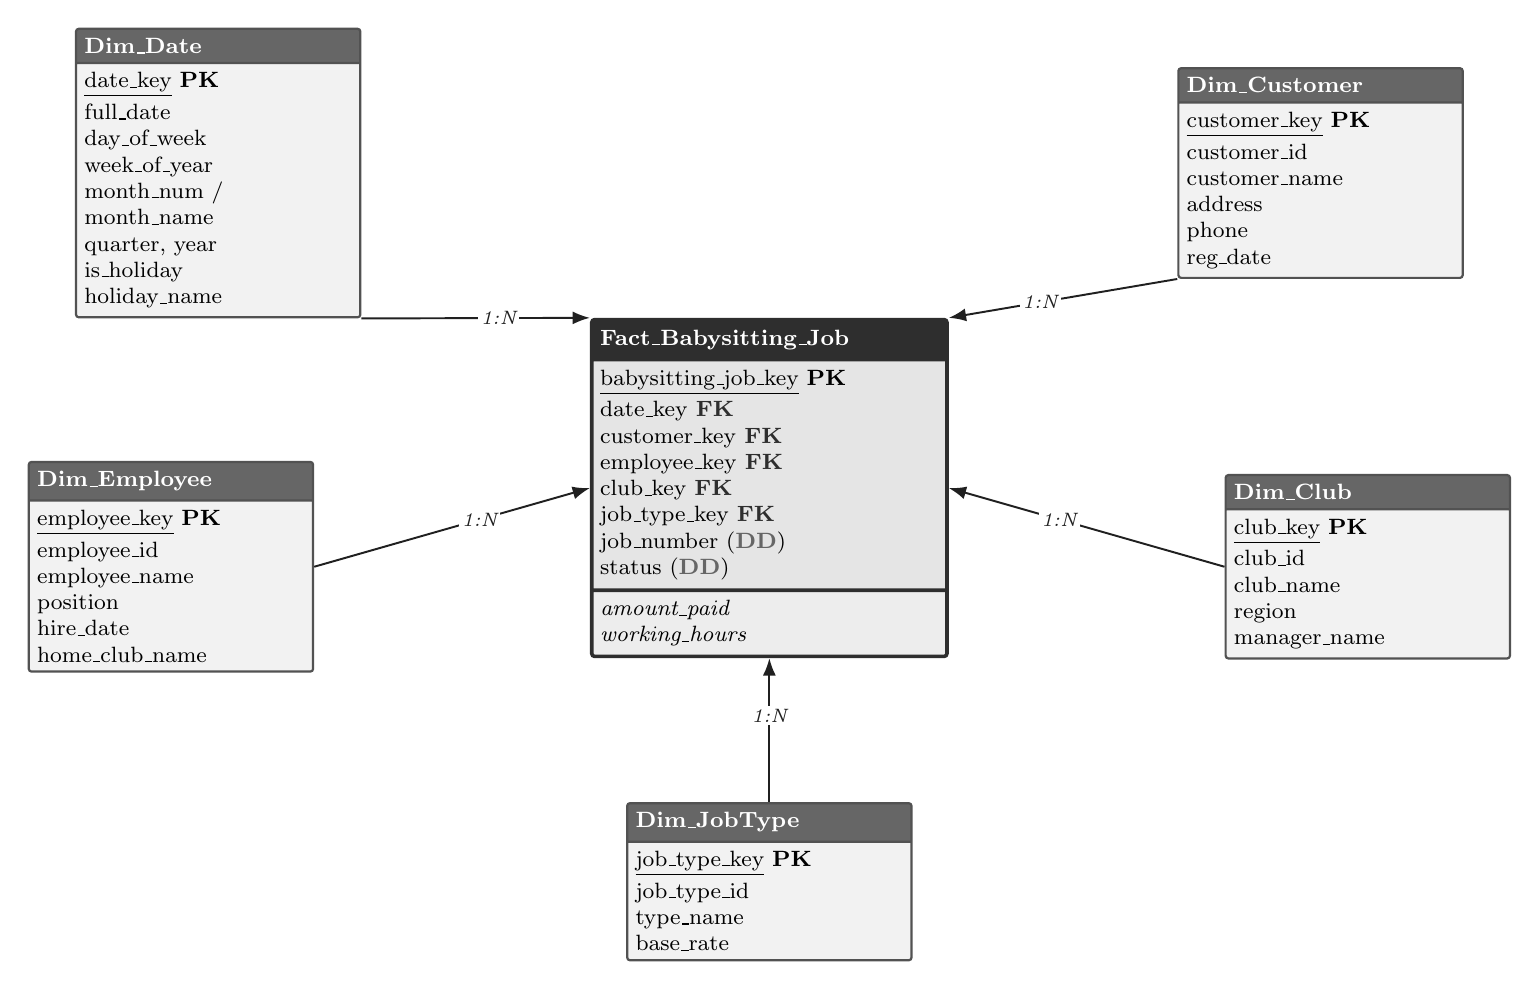
\begin{tikzpicture}[
  every node/.style={font=\footnotesize},
  dim/.style={draw=dimHead!80!black, line width=0.8pt, rounded corners=1pt,
      rectangle split, rectangle split parts=2,
      rectangle split part fill={dimHead, dimBody},
      text width=3.4cm, align=left, inner sep=3pt},
  facttbl/.style={draw=factHead, line width=1.3pt, rounded corners=1pt,
      rectangle split, rectangle split parts=3,
      rectangle split part fill={factHead, factBody, factBody!70!white},
      text width=4.3cm, align=left, inner sep=3pt},
  rel/.style={-{Latex[length=2.2mm]}, line width=0.7pt, factHead!70!black},
  hdr/.style={text=white}, lbl/.style={font=\scriptsize\itshape, fill=white, inner sep=1pt}
]
\node[facttbl] (fact) at (0,0) {
  \nodepart[hdr]{one}\textbf{Fact\_Babysitting\_Job}
  \nodepart{two}
    \underline{babysitting\_job\_key} \PK\\[2pt]
    date\_key \FK\\ customer\_key \FK\\ employee\_key \FK\\
    club\_key \FK\\ job\_type\_key \FK\\ job\_number (\DD)\\ status (\DD)
  \nodepart{three}\textit{amount\_paid}\\ \textit{working\_hours}};

\node[dim] (date) at (-7.0,4.0) {
  \nodepart[hdr]{one}\textbf{Dim\_Date}
  \nodepart{two}\underline{date\_key} \PK\\[2pt] full\_date\\ day\_of\_week\\ week\_of\_year\\
     month\_num / month\_name\\ quarter, year\\ is\_holiday\\ holiday\_name};
\node[dim] (cust) at (7.0,4.0) {
  \nodepart[hdr]{one}\textbf{Dim\_Customer}
  \nodepart{two}\underline{customer\_key} \PK\\[2pt] customer\_id\\ customer\_name\\ address\\ phone\\ reg\_date};
\node[dim] (emp) at (-7.6,-1.0) {
  \nodepart[hdr]{one}\textbf{Dim\_Employee}
  \nodepart{two}\underline{employee\_key} \PK\\[2pt] employee\_id\\ employee\_name\\ position\\ hire\_date\\ home\_club\_name};
\node[dim] (club) at (7.6,-1.0) {
  \nodepart[hdr]{one}\textbf{Dim\_Club}
  \nodepart{two}\underline{club\_key} \PK\\[2pt] club\_id\\ club\_name\\ region\\ manager\_name};
\node[dim] (jt) at (0,-5.0) {
  \nodepart[hdr]{one}\textbf{Dim\_JobType}
  \nodepart{two}\underline{job\_type\_key} \PK\\[2pt] job\_type\_id\\ type\_name\\ base\_rate};

\draw[rel] (date.south east) -- node[lbl,pos=0.6]{1:N} (fact.north west);
\draw[rel] (cust.south west) -- node[lbl,pos=0.6]{1:N} (fact.north east);
\draw[rel] (emp.east)        -- node[lbl,pos=0.6]{1:N} (fact.west);
\draw[rel] (club.west)       -- node[lbl,pos=0.6]{1:N} (fact.east);
\draw[rel] (jt.north)        -- node[lbl,pos=0.6]{1:N} (fact.south);
\end{tikzpicture}}
\end{center}
\vspace{2pt}
\noindent\small One central fact, five dimensions (a star). Each dimension links
to the fact 1:N via its surrogate key (\PK\ in the dimension, \FK\ in the fact);
\code{job\_number} and \code{status} are degenerate dimensions (\DD); measures sit
in the fact's lower partition.\normalsize

\end{document}
